\begin{frame}{Messpunkt}
	\begin{center}
		\includestandalone[keepaspectratio,scale=0.7]{tikz/baTopAngriffArp}
	\end{center}
	\note{
		Notes
	}
\end{frame}


\begin{frame}{ARP-Spoofing}
	\begin{center}
		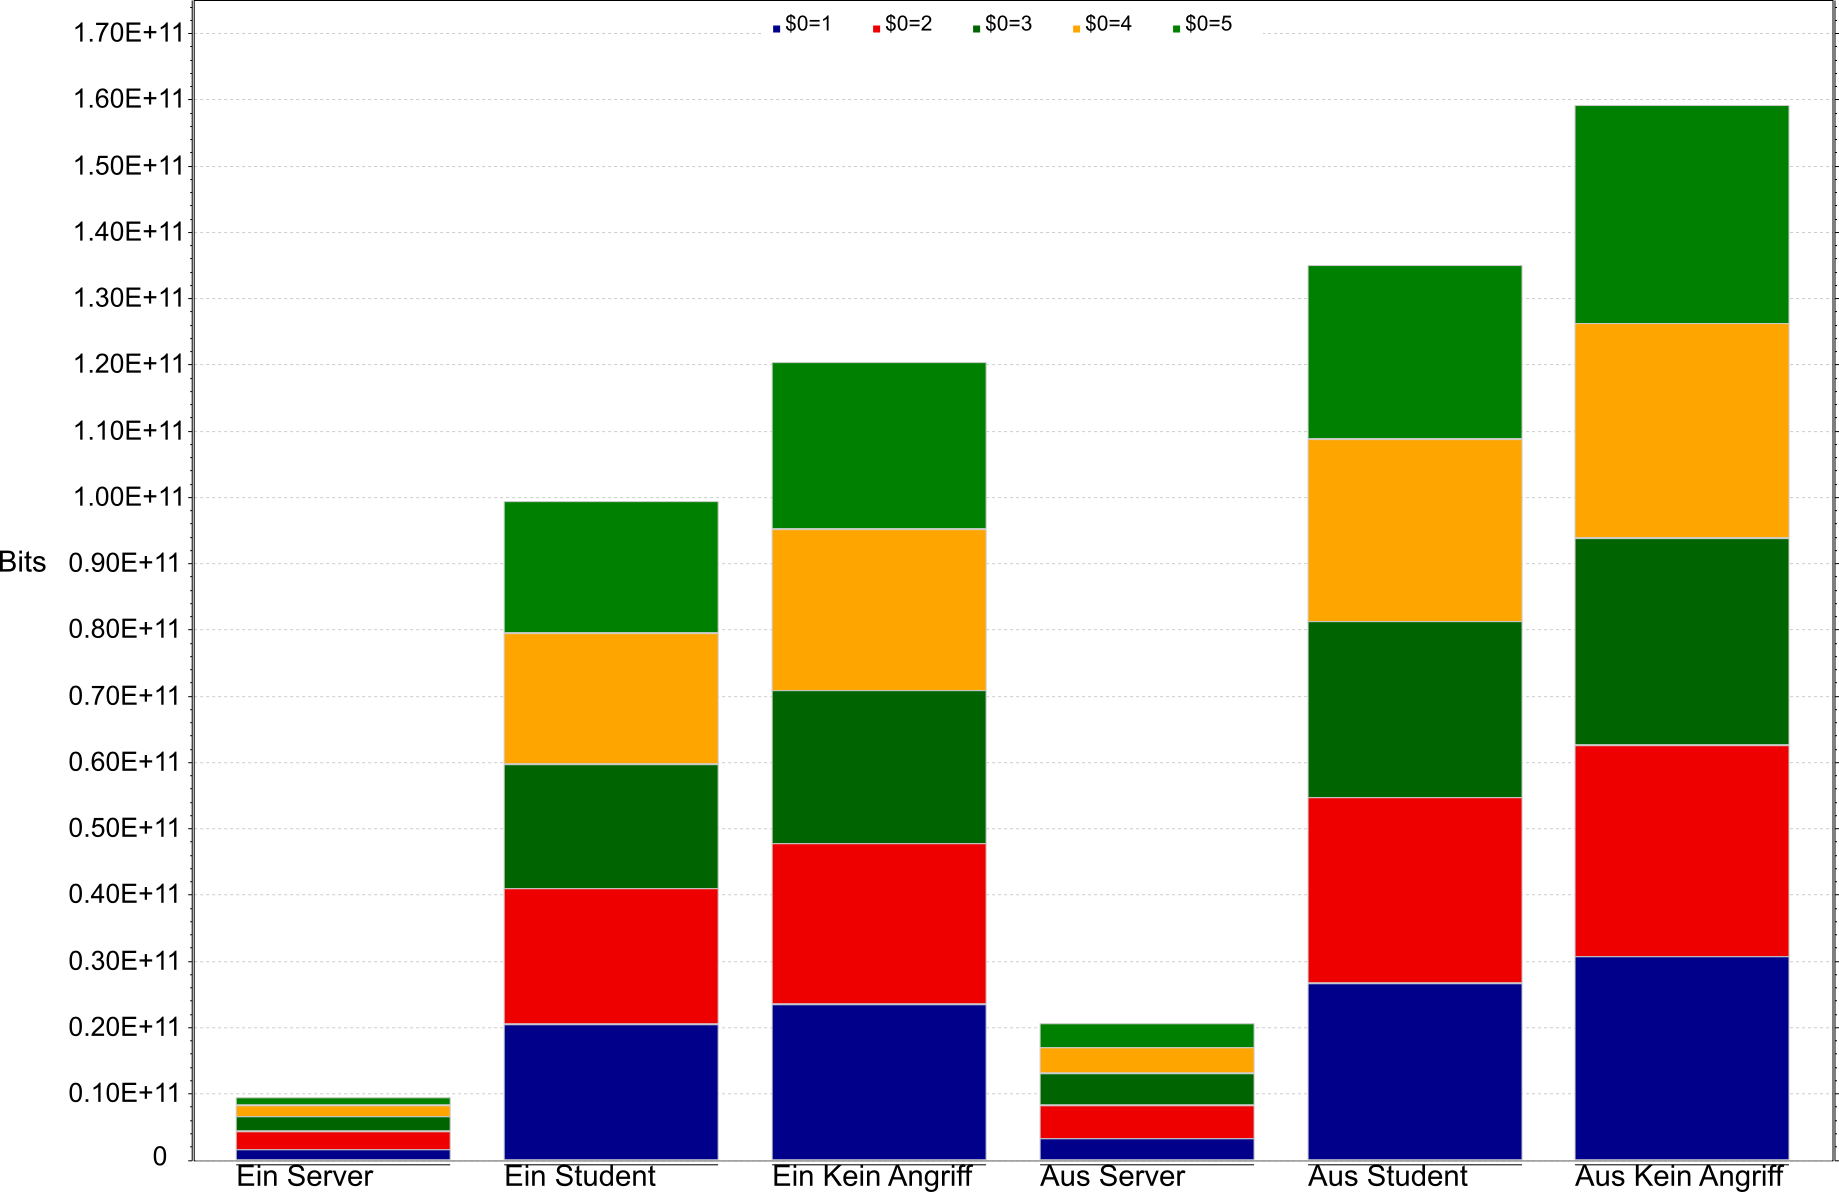
\includegraphics[keepaspectratio,
		width=\paperwidth,
		height=0.8\paperheight]{pic/arp/ArpBitIrb.png}
	\end{center}
	\note{
		Notes
	}
\end{frame}

\begin{frame}{SYN-Flooding}
	\begin{center}
		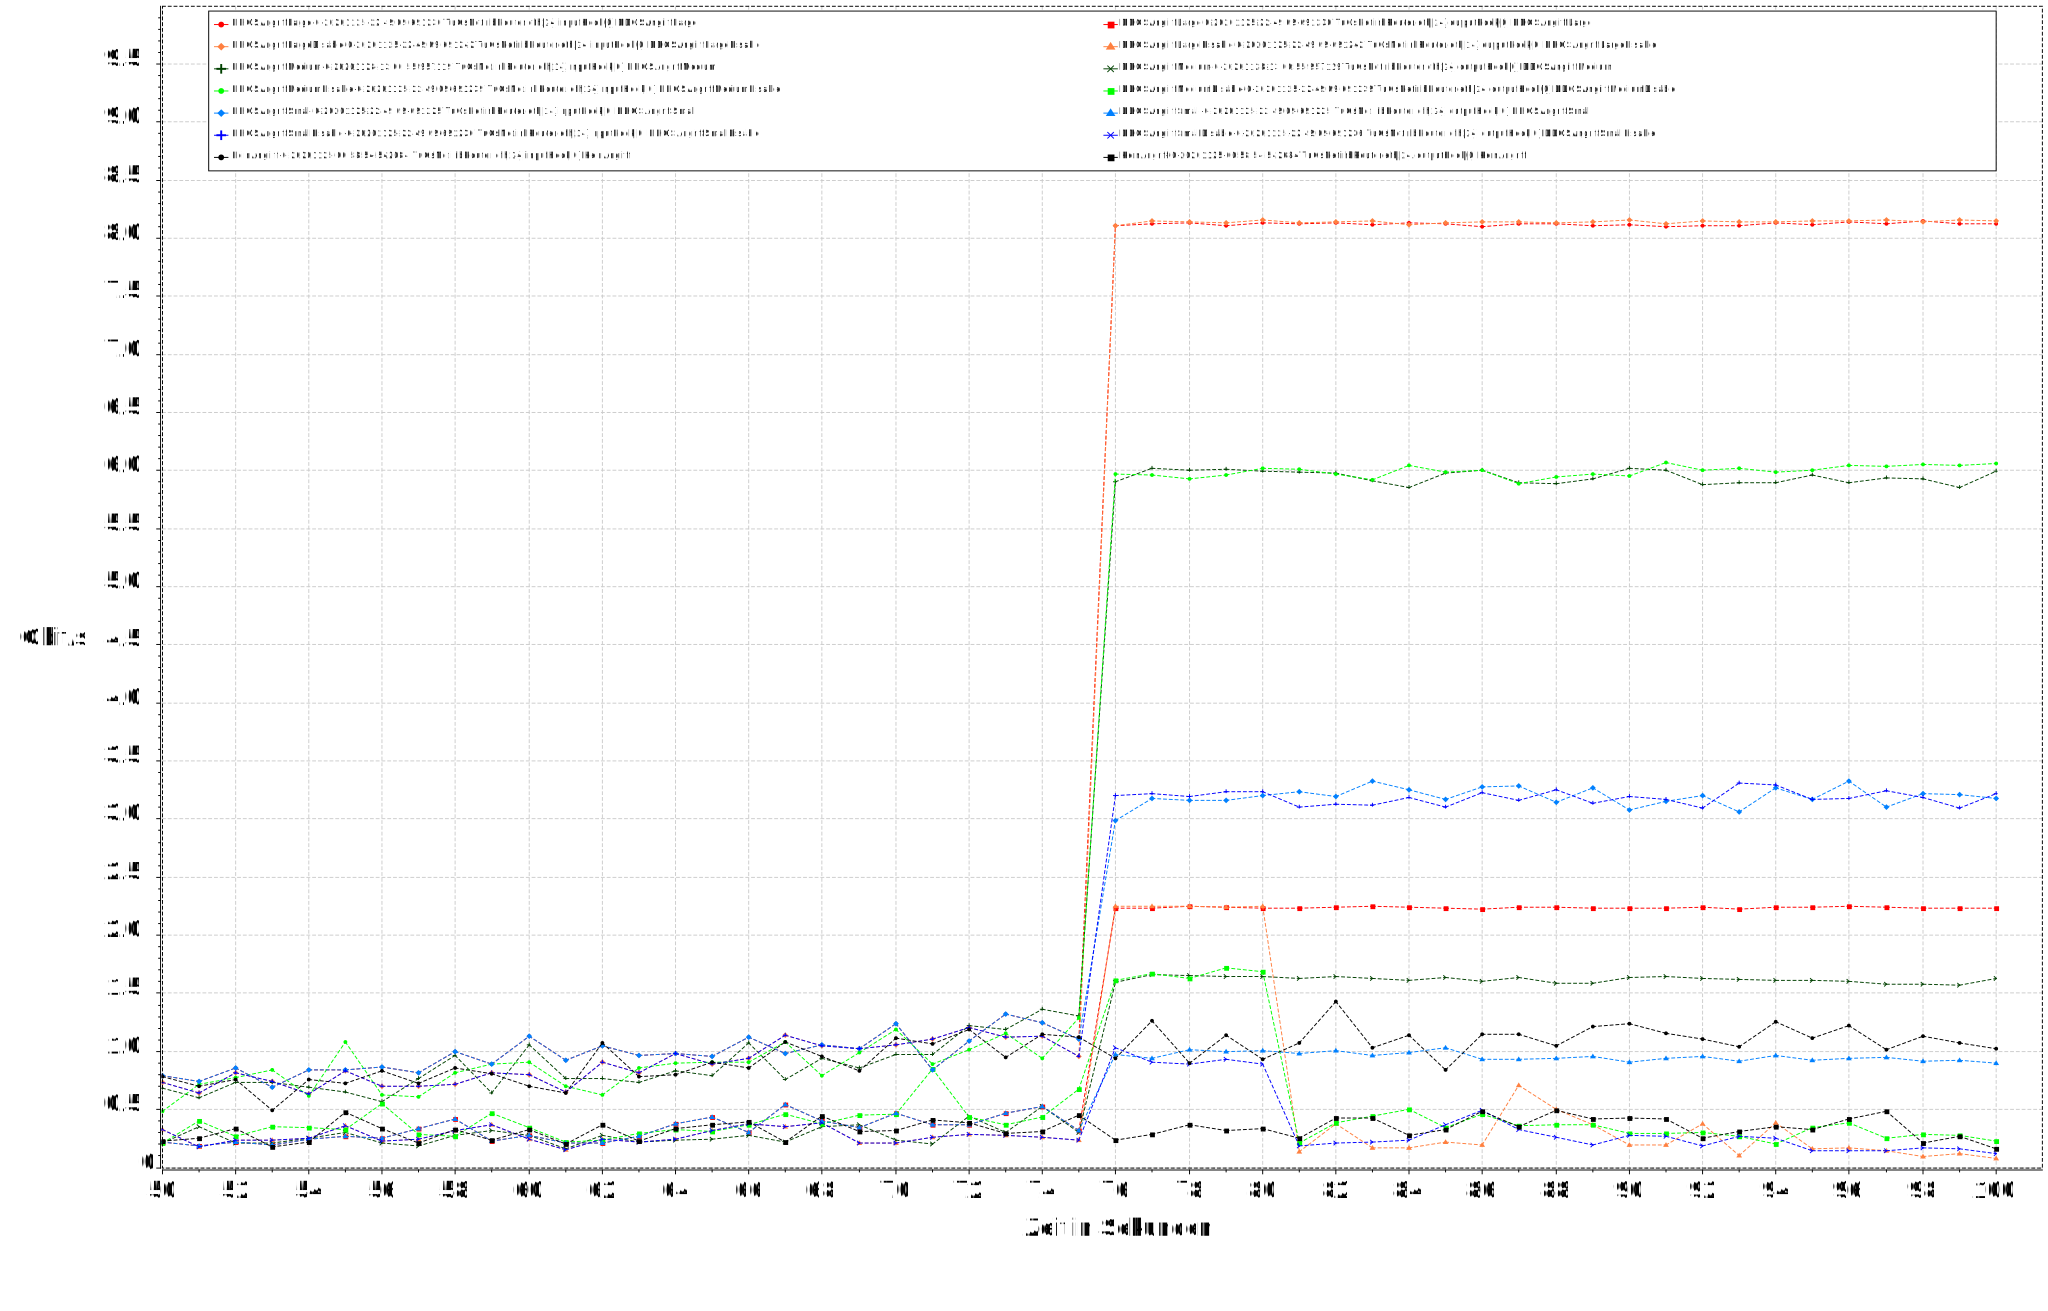
\includegraphics[keepaspectratio,
		width=\paperwidth,
		height=0.8\paperheight]{pic/dos/InternetRouterThruput}
	\end{center}
	\note{
		Notes
	}
\end{frame}

\begin{frame}{Messpunkt}
	\begin{center}
		
		\includestandalone[keepaspectratio,scale=0.7]{tikz/baTopAngriffPort}
	\end{center}
	\note{
		Notes
	}
\end{frame}

\begin{frame}{Firewall-Scanner}
	\begin{center}
		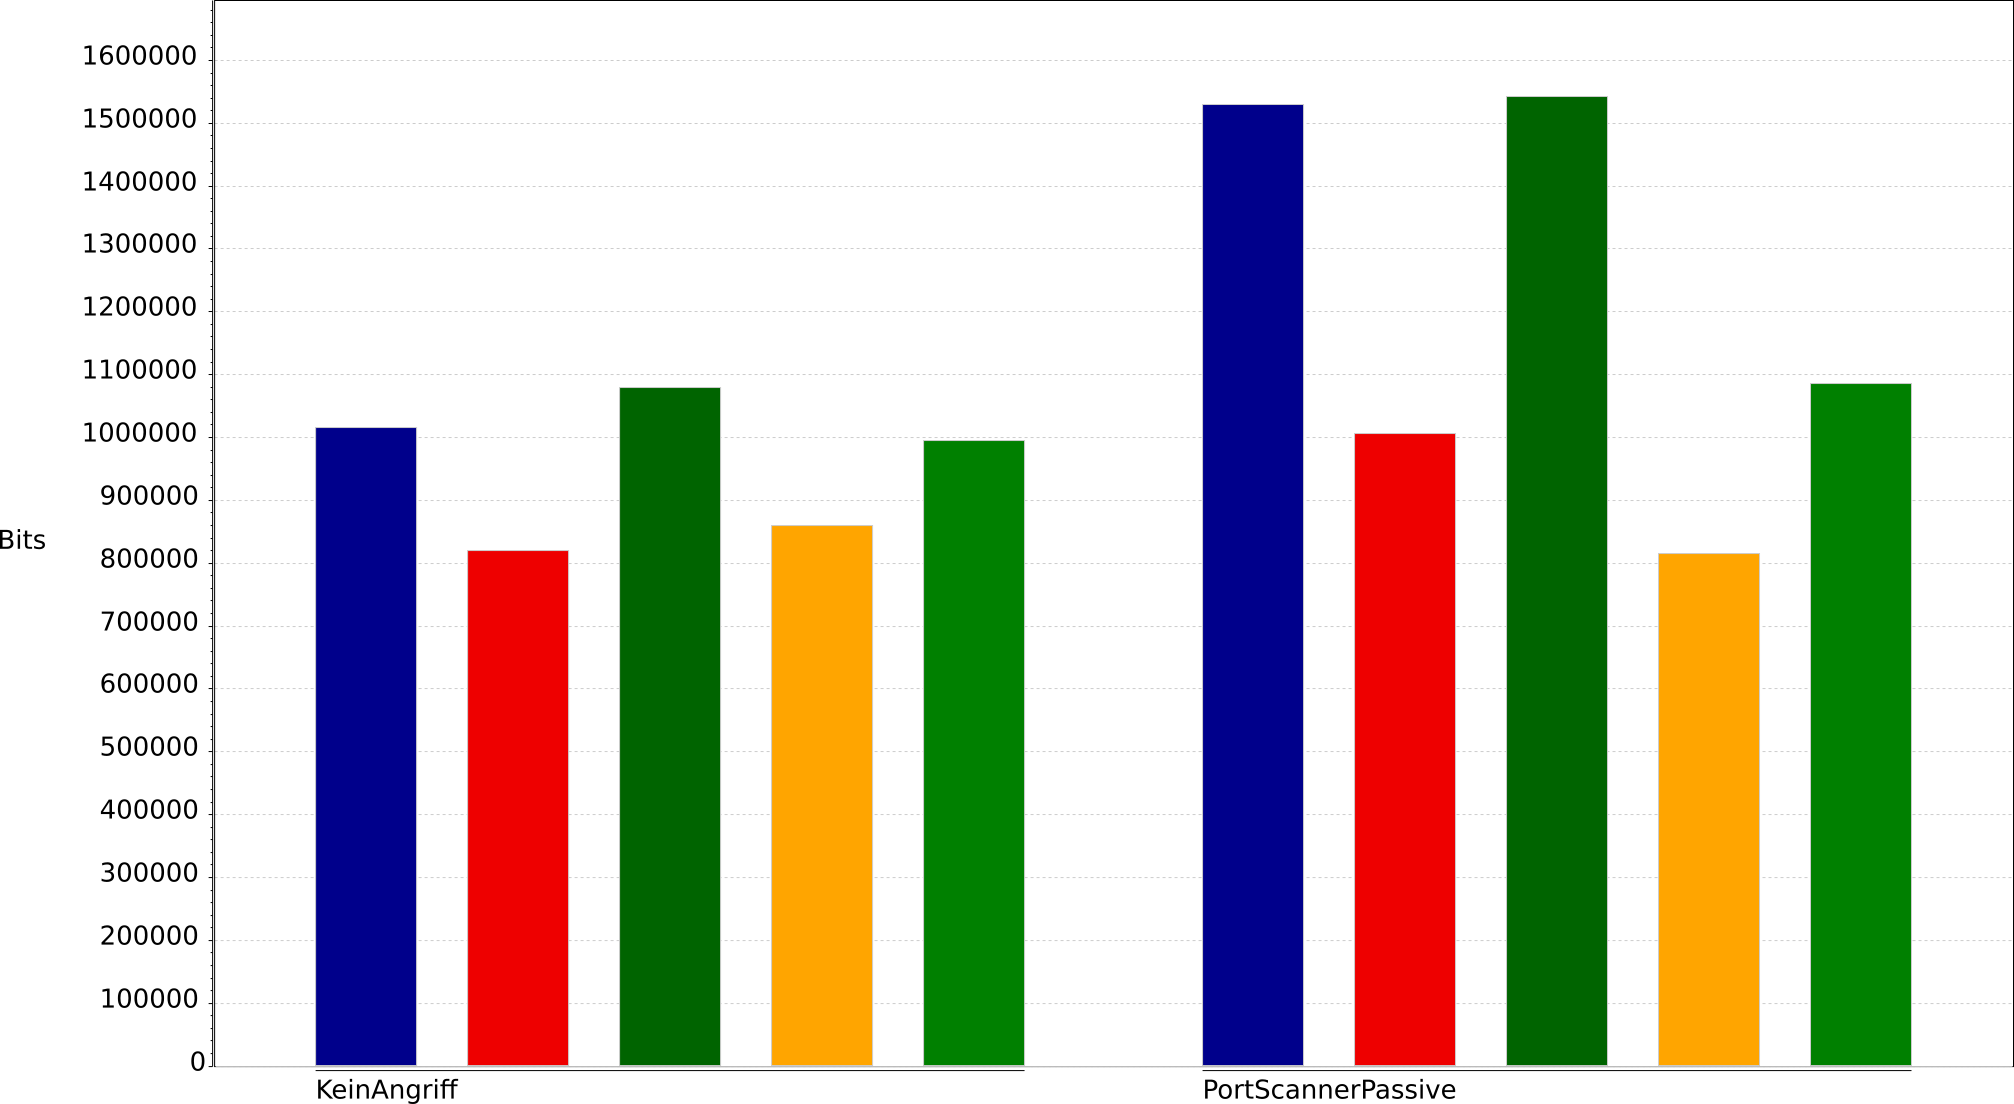
\includegraphics[keepaspectratio,
		width=\paperwidth, 
		height=0.8\paperheight]{pic/port/PortAngriffThruput.png}
	\end{center}
	\note{
		Notes
	}
\end{frame}

\begin{frame}{Zufall in OMNeT++}
	\begin{columns}[] 
		\begin{column}{0.5 \textwidth}
			\textbf{Implementierung des Zufalls}
			\begin{itemize}
				\item Jede Konfiguration besitzt ein Seed
				\item Seed kann festgelegt werden
				\item Zufallsgenerator erzeugt Sequenz aus Zahlen
				\begin{itemize}
					\item[$\Rightarrow$] Immer gleiche Reihenfolge
				\end{itemize}
			\end{itemize}
		\end{column}%
		\begin{column}{0.5 \textwidth}
			\begin{tiny}
				\begin{center}
					\includesvg[width=\textwidth]{pic/zufallTestKlein.svg}
				\end{center}
			\end{tiny}
		\end{column}
	\end{columns}
	\note{
		Notes
	}
\end{frame}
